\documentclass[10pt,a4paper]{amsart}
\usepackage{amsmath,amssymb,amsthm,graphicx}
\usepackage[margin=1in]{geometry}
\usepackage{amsmath, amssymb, amsthm}
\usepackage{mathtools} \usepackage{xcolor} \usepackage{bm} \usepackage{float}
\usepackage[colorlinks=true, linkcolor=black, citecolor=black,urlcolor=black, filecolor=black]{hyperref} \usepackage{tikz}

% ---------- Colorblind-friendly palette (Okabe--Ito) ----------
\definecolor{cbBlue}{RGB}{0,114,178}
\definecolor{cbVermillion}{RGB}{213,94,0}
\definecolor{cbOrange}{RGB}{230,159,0}
\definecolor{cbSkyBlue}{RGB}{86,180,233}
\definecolor{cbGreen}{RGB}{0,158,115}
\definecolor{cbYellow}{RGB}{240,228,66}
\definecolor{cbPurple}{RGB}{204,121,167}

% ---------- Theorem environments ----------
\theoremstyle{plain}
\newtheorem{theorem}{Theorem}[section]
\newtheorem{proposition}[theorem]{Proposition}
\newtheorem{lemma}[theorem]{Lemma}
\newtheorem{corollary}[theorem]{Corollary}
\newtheorem{conjecture}[theorem]{Conjecture}
\newtheorem{question}[theorem]{Question}
\theoremstyle{definition}
\newtheorem{definition}[theorem]{Definition}
\newtheorem{example}[theorem]{Example}
\newtheorem{remark}[theorem]{Remark}

% ---------- Symbol and operator macros ----------
\newcommand{\Z}{\mathbb{Z}}
\newcommand{\Q}{\mathbb{Q}}
\newcommand{\N}{\mathbb{N}}
\newcommand{\R}{\mathbb{R}}
\newcommand{\kk}{\Bbbk}
\newcommand{\M}{\mathcal{M}}
\newcommand{\hyp}{\Delta_{k,n}}
\newcommand{\Tri}{\mathcal{T}_{k,n}}
\newcommand{\dosp}{\mathsf{S}}
\newcommand{\triv}{\mathbf{1}}

\DeclareMathOperator{\des}{des}
\DeclareMathOperator{\typ}{type}
\DeclareMathOperator{\comp}{comp}
\DeclareMathOperator{\ccomp}{ccomp}
\DeclareMathOperator{\Hyp}{Hyp}
\DeclareMathOperator{\base}{base}
\DeclareMathOperator{\cEq}{cEq}
\DeclareMathOperator{\Stab}{Stab}
\DeclareMathOperator{\inv}{inv}
\DeclareMathOperator{\cDes}{cDes}
\DeclareMathOperator{\Des}{Des}
\DeclareMathOperator{\eq}{eq}
\DeclareMathOperator{\Eq}{Eq}
\DeclareMathOperator{\wind}{wind}
\DeclareMathOperator{\Ehr}{Ehr}
\DeclareMathOperator{\Hilb}{Hilb}
\DeclareMathOperator{\hDOSP}{hDOSP}
\DeclareMathOperator{\DOSP}{DOSP}
\DeclareMathOperator{\col}{color}
\DeclareMathOperator{\conv}{convex}
\DeclareMathOperator{\Ind}{Ind}
\DeclareMathOperator{\Pl}{Pl}
\DeclareMathOperator{\Sym}{Sym}
\DeclareMathOperator{\Hom}{Hom}
\DeclareMathOperator{\diag}{diag}
\DeclareMathOperator{\tr}{tr}
\DeclareMathOperator{\supp}{supp}
\DeclareMathOperator{\cdes}{cdes}
\DeclareMathOperator{\ceq}{ceq}
\DeclareMathOperator{\cmaj}{cmaj}
\DeclareMathOperator{\content}{content}
\DeclareMathOperator{\ch}{ch}
\title{Flag refinement of the hypersimplex h-star formula and Young-module interpretation}
\author{Yuhan Jiang}
\date{arxiv:2610.07451v1; CC BY 4.0}
\begin{document}
\maketitle
\noindent\textit{Editorial note.} Complete original mathematical paper91--873, all nonadjacent supporting proofs and unchanged main.bib retained. Authors retain responsibility for mathematics; no proof repair, added assumptions, independent author review or certification.\par\medskip
\noindent\textit{Editorial note.} Original flag-h and Young-module main statements form one combined refinement object. Their coprimality and cyclic-composition conventions remain exact; intermediate generating-function/contingency identities and direct consequences are full proof support, not extra counts.\par\medskip
\noindent\textit{Editorial note.} Focused public neighbor1001 concerns a different integral matroid Chow-ring tree-expansion theorem, not this hypersimplex alcove flag enumeration. No proof re-audit performed.\par\medskip
\noindent\textit{Allowed standard prerequisites (editorial).}\begin{itemize}
\item Hypersimplex alcove triangulations, decorated ordered partitions, cyclic flags and symmetric functions. Original k/n, cyclic composition, balanced coloring, flag h/f, Young module and gcd(k,n)=1 hypotheses retained; known Early-Kim theorem and alcove description remain explicitly cited. All source-local symmetric-function/bijection proofs supplied.. Complete original paper and main.bib retained; no independent verification, added hypotheses or proof reconstruction.
\end{itemize}\medskip
\section{Introduction}
The hypersimplex $ \hyp = \{ x \in [0,1]^n: \sum_i x_i = k\} $ is a $ (n-1) $ -dimensional polytope with $ \binom{n}{k}
$ vertices. The \emph{Ehrhart polynomial} $ \Ehr(P,t) $ of a lattice polytope $ P $ is defined such that
\[
	\Ehr(P,t) = |tP \cap \Z^n|, \qquad \text{ for }t \in \N.
\]
The \emph{ $ h^* $-polynomial} of $ P $ is defined by the generating function
\[
	\sum_{t \ge 0} \Ehr(P,t) z^t = \frac{h^*(P,z)}{(1-z)^{\dim(P)+1}}.
\]
Early conjectured a combinatorial formula for the $ h^* $-polynomial of $ \hyp $ in terms of \emph{hypersimplicial
  decorated ordered set partitions}, which was later proved by Kim~\cite{Kim2020}.
\begin{definition}\label{def:dosp}
	Let $(S_1, \dots, S_p)$ be an ordered set partition of $ [n] $ and $(s_1, \dots, s_p)$ be a composition of $k$.
	There is an equivalence relation on these pairs, defined by
	\[
		((S_1)_{s_1},(S_2)_{s_2},\dots,(S_p)_{s_p}) \sim
		((S_2)_{s_2},\dots,(S_p)_{s_p},(S_1)_{s_1}).
	\]
	A \emph{decorated ordered set partition}
	\begin{equation}\label{eq:dosp}
		\dosp = [((S_1)_{s_1},\dots,(S_p)_{s_p})]
	\end{equation}
	is an equivalence class of such pairs.
	A decorated ordered set partition is \emph{hypersimplicial} if $ 1 \leq s_i \leq |S_i|-1 $ for all $ i $. We denote the set of hypersimplicial decorated
	ordered set partitions of type $ (k,n) $ by $ \hDOSP(k,n) $. We call each $ S_i $ a block, place the blocks on a
	circle clockwise, and regard $ s_i $ as the clockwise distance between adjacent blocks $ S_i $ and $ S_{i+1} $. The
	\emph{winding number} of $ \dosp $ is defined as the number of times we wrap around the circle as we trace $ 1 \to
		2 \to \cdots \to n \to 1 $ clockwise.
\end{definition}
\begin{figure}[H]
	\centering
	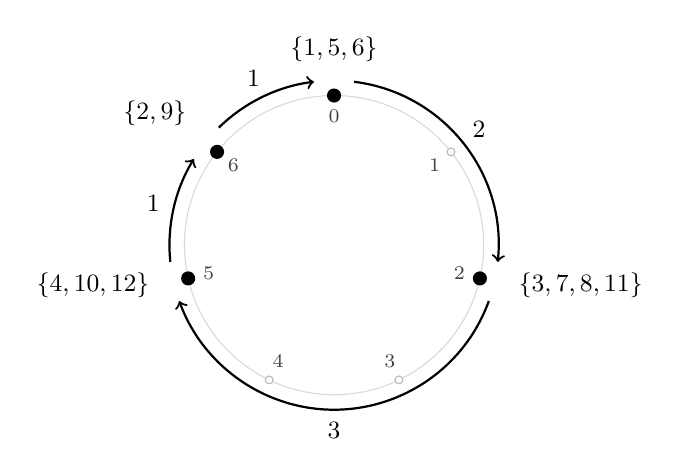
\begin{tikzpicture}[scale=1.9]
	\draw[gray!30] (0,0) circle (1);
	\foreach \p in {0,...,6}{
			\node[circle,draw=gray!55,fill=white,inner sep=1pt] at ({90-360*\p/7}:1) {};
			\node[black!75,font=\scriptsize] at ({90-360*\p/7}:0.86) { $ \p $ }; }
	\foreach \p in {0,2,5,6}{
			\node[circle,fill=black,inner sep=1.8pt] at ({90-360*\p/7}:1) {}; }
	\node[font=\small,anchor=south]      at ({90}:1.16)        { $ \{1,5,6\} $ };
	\node[font=\small,anchor=west]       at ({90-720/7}:1.20)  { $ \{3,7,8,11\} $ };
	\node[font=\small,anchor=east]       at ({90-1800/7}:1.20) { $ \{4,10,12\} $ };
	\node[font=\small,anchor=south east] at ({90-2160/7}:1.18) { $ \{2,9\} $ };
	\draw[->,thick] ({90-7}:1.10) arc ({90-7}:{90-720/7+7}:1.10);
	\node[font=\small] at ({90-360/7}:1.24) { $ 2 $ };
	\draw[->,thick] ({90-720/7-7}:1.10) arc ({90-720/7-7}:{90-1800/7+7}:1.10);
	\node[font=\small] at ({90-1260/7}:1.24) { $ 3 $ };
	\draw[->,thick] ({90-1800/7-7}:1.10) arc ({90-1800/7-7}:{90-2160/7+7}:1.10);
	\node[font=\small] at ({90-1980/7}:1.24) { $ 1 $ };
	\draw[->,thick] ({90-2160/7-7}:1.10) arc ({90-2160/7-7}:{90-360+7}:1.10);
	\node[font=\small] at ({90-2340/7}:1.24) { $ 1 $ };
	\end{tikzpicture}
	\caption{The decorated ordered set partition $
			(\{1,5,6\}_2,\{3,7,8,11\}_3,\{4,10,12\}_1,\{2,9\}_1) $ of type $ (7,12) $ with winding number $ 5 $.}\label{fig:dosp}
\end{figure}

\begin{remark}
	Let $(S_1,\dots,S_p)$ be an ordered set partition of $[n]$, and $(s_1,\dots,s_p)$ be a composition of $k$.
	For a set $S$, let $x_S = \sum_{i \in S} x_i$.
	Derksen and Fink~\cite{DerksenFink} showed that the cones determined by the inequalities
	\begin{equation}
		\begin{aligned}
			x_{S_1}          & \leq s_1 \\
			x_{S_1 \cup S_2} & \leq s_1+s_2 \\
			                 & \vdots \\
			x_{[n]}          & \leq k.
		\end{aligned}
	\end{equation}
	form a basis of the valuative ring of matroids on the ground set $[n]$ of rank $k$.
\end{remark}

\begin{theorem}[\cite{Early2017,Kim2020}]\label{thm:earlykim}
	The $ h^* $ -polynomial of the hypersimplex $ \hyp $ is given by
	\[
		h^*(\hyp,z) = \sum_{\dosp \in \hDOSP(k,n)} z^{\wind(\dosp)}.
	\]
\end{theorem}

\begin{figure}
	\centering
	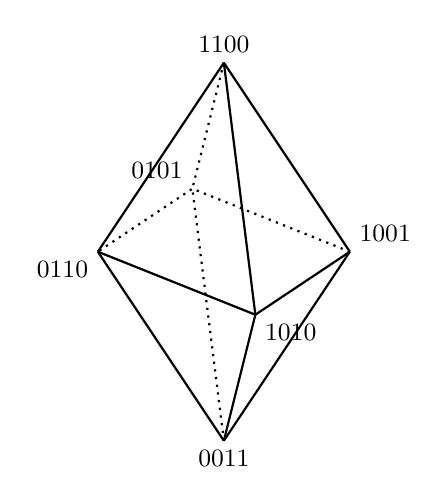
\begin{tikzpicture}[scale=.8,every node/.style={font=\small}]
	\coordinate (A) at (0,1);
	\coordinate (B) at (2.5,0);
	\coordinate (C) at (4,1);
	\coordinate (D) at (1.5,2);

	% Define the coordinate for the apex of the pyramid
	\coordinate (Apex) at (2,4);
	\coordinate (Bot) at (2,-2);

	% Draw the base of the pyramid
	\draw[thick] (A) -- (B) -- (C);
	\draw[thick,dotted] (C) -- (D) --(A);

	% Draw the edges from the apex to the base vertices
	\draw[thick] (Apex) -- (A);
	\draw[thick] (Apex) -- (B);
	\draw[thick] (Apex) -- (C);
	\draw[thick,dotted] (Apex) -- (D);
	\draw[thick] (Bot) -- (A);
	\draw[thick] (Bot) -- (B);
	\draw[thick] (Bot) -- (C);
	\draw[thick,dotted] (Bot) -- (D);

	% Label the base vertices
	\node[below left] at (A) {0110};
	\node[below right] at (B) {1010};
	\node[above right] at (C) {1001};
	\node[above left] at (D) {0101};

	% Label the apex
	\node[above] at (Apex) {1100};
	\node[below] at (Bot) {0011};
	\end{tikzpicture}
	\caption{The hypersimplex $ \Delta_{2,4} $.}\label{fig:d24}
\end{figure}

\begin{figure}
	\centering
	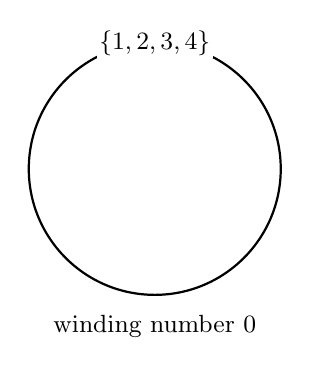
\begin{tikzpicture}[scale=.8, every node/.style={fill=white, inner sep=1pt, font=\small},
	arc/.style={thick, ->, >=Stealth}]
	\draw[thick] (0,0) circle (2);
	\node (A) at (90:2) { $ \{1,2,3,4\} $ };
	\node at (0,-2.5) {winding number $ 0 $ };
	\end{tikzpicture}
	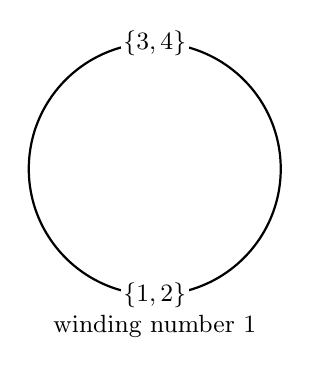
\begin{tikzpicture}[scale=.8,every node/.style={fill=white, inner sep=1pt, font=\small},
	arc/.style={thick, ->, >=Stealth}]
	\draw[thick] (0,0) circle (2);
	\node (A) at (270:2) { $ \{1,2\} $ };
	\node (B) at (90:2) { $ \{3,4\} $ };
	\node at (0,-2.5) {winding number $ 1 $ };
	\end{tikzpicture}
	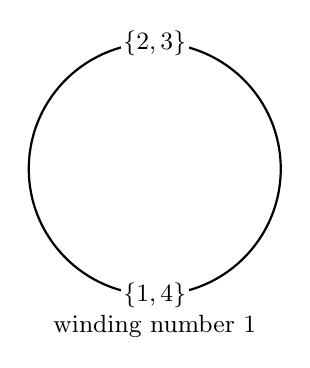
\begin{tikzpicture}[scale=.8,every node/.style={fill=white, inner sep=1pt, font=\small},
	arc/.style={thick, ->, >=Stealth}]
	\draw[thick] (0,0) circle (2);
	\node (A) at (270:2) { $ \{1,4\} $ };
	\node (B) at (90:2) { $ \{2,3\} $ };
	\node at (0,-2.5) {winding number $ 1 $ };
	\end{tikzpicture}
	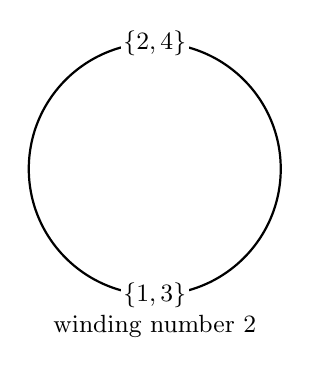
\begin{tikzpicture}[scale=.8,every node/.style={fill=white, inner sep=1pt, font=\small},
	arc/.style={thick, ->, >=Stealth}]
	\draw[thick] (0,0) circle (2);
	\node (A) at (270:2) { $ \{1,3\} $ };
	\node (B) at (90:2) { $ \{2,4\} $ };
	\node at (0,-2.5) {winding number $ 2 $ };
	\end{tikzpicture}
	\caption{ $ \hDOSP(2,4) $.}\label{fig:dosp24}
\end{figure}

\begin{example}\label{ex:d24}
	The hypersimplex $ \Delta_{2,4} $
	is the octahedron shown in Figure~\ref{fig:d24}.
	The hypersimplicial decorated ordered set partitions of type $ (2,4) $
	are shown in Figure~\ref{fig:dosp24}, and we have
	\[
		h^*(\Delta_{2,4},z) = 1 + 2z + z^2.
	\]
\end{example}

\subsection{Balanced complexes and flag numbers}\label{ss:balanced-flag}
There is a \emph{unimodular triangulation} of the hypersimplex $\hyp$ by \emph{alcoves}, studied by Postnikov and Lam
in~\cite{alcove1}. The \emph{alcove triangulation complex} of $\hyp$, denoted $\Tri$, is the simplicial complex with
vertex set $\binom{[n]}{k}$, and maximal faces called \emph{alcoves} (See Section~\ref{sec:triangulation}). Since
$\Tri$ is unimodular, Stanley's result in~\cite{stanley80} implies that \[h^*_d(\hyp) = h_d(\Tri).\] Our main result gives a refinement of Theorem~\ref{thm:earlykim} by flag numbers introduced by Stanley in the study
   of balanced complexes~\cite{Stanley1979}.

Let $\Delta $ be a simplicial complex on a vertex set $ V $. A face with $ i+1 $ elements is an \emph{ $ i $-face} and
has $ \dim F=i $; if $ \delta=\max\{\dim F:F\in\Delta\} $ then $ \Delta $ is a \emph{$ \delta $-complex} and $
\dim\Delta=\delta $, and $ \Delta $ is \emph{pure} if every maximal face is a $ \delta $-face~\cite[\S1]{Stanley1979}.

\begin{definition}[{\cite[\S2]{Stanley1979}}]\label{def:balanced}
	A \emph{balanced complex} of type $ (a_1,\dots,a_m) $ is a pair $ (\Delta,\pi) $ such that $ \Delta $ is a pure $ \delta $
	-complex on a vertex set $ V $ and $\pi=(V_1,\ldots, V_m)$ is an ordered set partition of $ V $
	such that for every maximal face $ F\in\Delta $ and every $ i\in[m] $, we have $ |F\cap V_i|=a_i $. Hence $
		a_1+\cdots+a_m=\delta+1 $.
	A balanced complex of type $ (1,1,\dots,1) $
	is \emph{completely balanced}.
\end{definition}

\begin{definition}[{\cite[\S3]{Stanley1979}}]\label{def:flag}
	Let $ (\Delta,\pi) $
	be completely balanced with $\pi = (V_1, \ldots,V_m)$.The \emph{color} of a vertex $ x\in V_i $ is $ \col(x)=i $, and the \emph{type} of a face $ F\in\Delta $ is
	\begin{equation}
		\typ(F)=\{\col(x):x\in F\}\subseteq[m].
	\end{equation}
	For $ S\subseteq[m] $ the \emph{flag $ f $-number} and the \emph{flag $ h $-number} of $ \Delta $ are
	\begin{equation}\label{eq:flagnumbers}
		f_S(\Delta)=\#\{F\in\Delta:\typ(F)=S\},\qquad
		h_S(\Delta)=\sum_{T\subseteq S}(-1)^{|S\setminus T|}f_T(\Delta).
	\end{equation}
\end{definition}

\begin{lemma}[Eq.6,\cite{Stanley1979}]
	If $\Delta$ is a completely balanced complex, then
	\begin{equation}\label{eq:flagh}
		h_d(\Delta)=\sum_{|S|=d} h_S(\Delta).
	\end{equation}
\end{lemma}

\subsection{Cyclic compositions and cyclic words}
A \emph{(resp.\ weak) composition} of $n$ with $p$ parts is a vector $(\alpha_1,\dots,\alpha_p)$ of (resp.\
nonnegative) positive integers such that $\sum_{i=0}^{p-1}\alpha_i = n$, denoted $\alpha \models n$. There is an
equivalence relation on (weak) compositions of $ n $ with $ p $ parts, induced by
\[
	(\alpha_1,\dots,\alpha_p) \sim \alpha^{(i)}:= (\alpha_i,\dots,\alpha_p,\alpha_1\dots,\alpha_{i-1}).
\]
The equivalence class under this relation is called a \emph{cyclic composition}, denoted $ [\alpha] $.

\begin{definition}
	For each subset $ S \subseteq [n] $ and for each $i \in S$, we associate a cyclic composition, denoted
	$\comp^{(i)}(S)$. We draw the points in $S$ clockwise on a circle, so that they cut the circle into $ |S| $ arcs. Let
	$\comp^{(i)}(S)_j$ be the arc length of the $j$-th arc clockwise after $i$. These arc lengths form a cyclic composition
	of $n$. The set $\{\comp^{(i)}(S): i \in S\}$ forms an equivalence class of compositions, which we denote by $\ccomp(S)$.
	Conventionally, let $\comp(S):= \comp^{\min S}(S)$.
\end{definition}

\begin{figure}
	\centering
	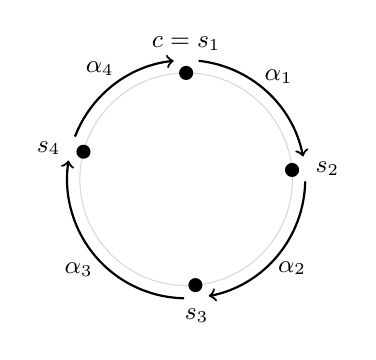
\begin{tikzpicture}[scale=1.35]
	\draw[gray!30] (0,0) circle (1);
	\foreach \a in {90, 5, -85, 165}{
			\node[circle,fill=black,inner sep=1.8pt] at (\a:1) {}; }
	\node[font=\small,anchor=south] at (90:1.12) { $ c=s_1 $ };
	\node[font=\small,anchor=west] at (5:1.13) { $ s_2 $ };
	\node[font=\small,anchor=north] at (-85:1.13) { $ s_3 $ };
	\node[font=\small,anchor=east] at (165:1.13) { $ s_4 $ };
	\draw[->,thick] (84:1.12) arc (84:11:1.12);
	\node[font=\small] at (48:1.30) { $ \alpha_1 $ };
	\draw[->,thick] (-1:1.12) arc (-1:-79:1.12);
	\node[font=\small] at (-40:1.30) { $ \alpha_2 $ };
	\draw[->,thick] (-91:1.12) arc (-91:-189:1.12);
	\node[font=\small] at (-140:1.32) { $ \alpha_3 $ };
	\draw[->,thick] (159:1.12) arc (159:96:1.12);
	\node[font=\small] at (128:1.32) { $ \alpha_4 $ };
	\end{tikzpicture}
	\caption{Reading the gaps of $
			S=\{s_1<s_2<s_3<s_4\}\subseteq\Z/n\Z $
: walking clockwise from $ c=s_1 $, the points of $ S $ appear in the order $ s_1,s_2,s_3,s_4 $, and $ \alpha_i $
		is the number of steps of the $ i $-th arc, giving $
			\comp^{c}(S)=(\alpha_1,\alpha_2,\alpha_3,\alpha_4)$.}\label{fig:comp}
\end{figure}

Let $ w:\Z/n\Z \to [k] $ be a word of length $n$ and alphabet $[k]$ for some positive integer $k$.
Following~\cite{magicnumber}, we define the \emph{cyclic descents} of $w$ as
\begin{equation}\label{eq:cdes}
	\cDes(w):=\{j\in\Z/n\Z:w(j)>w(j+1)\},\qquad \cdes(w) = |\cDes(w)|
\end{equation}
The \emph{content} of $ w $
is the \emph{weak} composition
\begin{equation}
	\content(w):= (|w^{-1}(1)|,\dots,|w^{-1}(k)|).
\end{equation}

\begin{definition}\label{def:hypersimplicial}
	Let $\alpha$ be a weak composition with $k$ parts.
	Viewing $\alpha: \Z/k\Z \to \Z_{\geq 0}$, we say that $\alpha \models n$ is \emph{hypersimplicial} if every positive entry satisfies $ \alpha_i > 1 $ and is
	followed by at most $ \alpha_i - 1 $ zeros on the circle.
	A cyclic word is \emph{hypersimplicial} if it has
	hypersimplicial content.
\end{definition}
Let $w$ be a cyclic word $\Z/n\Z \to [k]$. For $ p \in \Z/k\Z $, define the \emph{$p$-shift} of $ w $ as the cyclic word
\begin{equation}\label{eq:pshift}
	w^{(p)}(i) = w(i) - p \mod k.
\end{equation}

\begin{definition}\label{def:reading_word}
	The \emph{reading word} of an ordered set partition$(S_1,\dots,S_p)$ is the cyclic word $ w $ defined by
	\begin{equation}\label{eq:reading-osp}
		w(i)= j \text{ if } i \in S_j.
	\end{equation}
\end{definition}
For a decorated ordered set partition in the form~\eqref{eq:dosp}, choose the representative such that $n \in S_1$, and
define $w_{\dosp}$ as the reading word of this representative. Let $\cDes(\dosp):= \cDes(w_{\dosp})$.

\subsection{Main results}\label{ss:main_results}
Our first main result is a refinement of Early--Kim's theorem by giving a combinatorial formula for Stanley's flag $ h
$-numbers of the alcove triangulation complex.

\begin{theorem}\label{thm:hmain}
	Let $ \Tri $ be the triangulation complex of $ \hyp $.
	Then, for each cyclic composition $ \alpha $, we have
	\begin{equation}
		\sum_{S: \ccomp(S) = [\alpha]} h_S(\Tri) = \left| \left\{ \dosp \in \hDOSP(k,n): \ccomp(\cDes(\dosp)) = [\alpha] \right\}\right|.
	\end{equation}
\end{theorem}


Our second result gives a representation theoretic interpretation of the flag $ f $-numbers. Let $ \alpha =
(\alpha_1,\dots,\alpha_r) $ be a weak composition of $ n $. The \emph{Young subgroup} is $ S_\alpha \cong S_{\alpha_1}
\times \cdots \times S_{\alpha_r} $, and the \emph{Young permutation module} of $\alpha$ is $ M^\alpha \cong
\Ind_{S_\alpha}^{S_n} \triv $, the $ S_n $ -module on the ordered set partitions $ (B_1,\dots,B_r) $ of $ [n] $ with $
|B_i| = \alpha_i $. The Frobenius character of $ M^\alpha $ is $ \ch M^{\alpha} = h_\alpha $, the complete homogeneous
symmetric function. Let
\begin{equation}
	\label{eq:Mkn} \M_{k,n} = \bigoplus_{\lambda \text{ hypersimplicial}} M^\lambda.
\end{equation}

\begin{theorem}\label{thm:repmain}
	Let $ \gcd(k,n)=1 $ and let $ S $
	be a nonempty subset of $ [n] $ with $\ccomp(S) = [\alpha]$. Then
	\begin{equation}
		k \, f_S(\Tri) = \dim \Hom_{S_n}(M^{\alpha}, \M_{k,n})
	\end{equation}
\end{theorem}


\subsection*{Organization}
In Section~\ref{sec:triangulation}, we introduce the alcoved triangulation of the hypersimplices. In
Section~\ref{sec:symm}, we prove symmetric function identities for the generating functions of the statistics we are
interested in. In Section~\ref{sec:hypwords}, we prove our main result.
\subsection*{Acknowledgements}
We thank Nick Early, Elisabeth Bullock, Donghyun Kim, Lauren Williams, and Sylvie Corteel for helpful discussion.


\section{The alcove triangulation}\label{sec:triangulation}

We introduce the alcove triangulation of the hypersimplex. Lam and Postnikov~\cite{alcove1} showed that the maximal
faces of $ \Tri $ are parametrized by minimal \emph{circuits}. Parisi, Sherman-Bennett, Tessler, and
Williams~\cite{magicnumber} showed that the circuits can be described as the cyclic descents set of permutations.

\begin{definition}[\cite{alcove1}]
	A sequence $ (I_1,\dots,I_n) $ of $ k $ -subsets of $ [n] $
	is a \emph{circuit} if for each $ i \in \Z/n\Z $, there exists $ j \in \Z/n\Z $ such that $
		I_{i+1} = I_i \setminus \{j\} \cup \{j+1\} $.
\end{definition}

\begin{theorem}[\cite{alcove1,magicnumber}]\label{thm:max_face}
	If $ (I_0,\dots,I_{n-1}) $
	is a maximal face in $ \Tri $
, then there exists a permutation $ w \in S_n $ with $ \cdes(w) = k $ such that  for any $p \in \Z/n\Z$, we have
	\begin{equation}\label{eq:circuit}
		I_{p} = I_{p-1} \setminus \{w^{-1}(p)-1\} \cup \{w^{-1}(p)\}
	\end{equation}
	for all $p \in \Z/n\Z$. Moreover, we may take $w(n)=1$ and
	\begin{equation}\label{eq:cDescirc}
		I_p = \cDes\left(w^{(p)}\right).
	\end{equation}
\end{theorem}

\begin{table}
	\begin{tabular}{|c|c|}
		\hline
		$w$  & $(I_0,\dots,I_3)$ \\
		\hline
		4312 & (12,13,14,24)     \\
		\hline
		4213 & (12,13,23,24)     \\
		\hline
		4231 & (13,14,24,34)     \\
		\hline
		4132 & (13,23,24,34)     \\
		\hline
	\end{tabular}
	\caption{The permutations and vertex sets indexing simplices in the hypersimplex $\Delta_{2,4}$.}\label{tab:d24}
\end{table}

\begin{example}\label{ex:maxface}
	In Figure~\ref{fig:d24}, the four simplices triangulating the hypersimplex $\Delta_{2,4}$ are shown in Table~\ref{tab:d24}.
	Take the second row in that table where $w^{(0)} = 4213$ with $\cDes(w^{(0)}) = \{1,2\}$. We have
	\begin{align*}
		w^{(1)} & = 3142, & \cDes(w^{(1)}) = \{1,3\}, \\
		w^{(2)} & = 2431, & \cDes(w^{(2)}) = \{2,3\}, \\
		w^{(3)} & = 1324, & \cDes(w^{(3)}) = \{2,4\}.
	\end{align*}
\end{example}

\begin{theorem}\label{thm:coloring}
	The alcove triangulation complex $ \Tri $ of $ \hyp $
	is completely balanced with respect to the coloring $
		\col(I):\equiv \sum_{i \in I} i \bmod n$.
\end{theorem}

\begin{proof}
	Suppose $F$ is a maximal face with circuits $(I_0,\dots,I_{n-1})$, then \[\col(I_{p}) \equiv \col(I_{p-1}) + 1 \bmod n, \qquad \text{ for any }p \in \Z/n\Z, \] so all the vertices of $F$ are of different colors, and each color appears only once. Any lower dimensional face is
    contained in a maximal face, and this property is inherited.
\end{proof}

Let $ \Z/n\Z $ acts on each $ S \subseteq [n] $ by
\begin{equation}
	S + j:= \{s + j \bmod n \colon s \in S\}, \qquad \text{ for each } j \in \Z/n\Z.
\end{equation}
\begin{proposition}
	Let $d = \gcd(k,n)$. For every $S \subseteq \Z/n\Z$, the flag numbers satisfy $f_S(\Tri) = f_{S+k}(\Tri)$ and $h_S(\Tri) = h_{S+k}(\Tri)$.
\end{proposition}
\begin{proof}
	Consider the rotation of the $n$-coordinates
	\[
		\rho: \R^n \to \R^n, (x_1,\dots,x_n) \mapsto
		(x_2,\dots,x_{n},x_1)
	\]
	which preserves the alcove triangulation. Then $\typ(\rho F) = \typ(F) + k$ and $f_S(\Tri) = f_{S+k}(\Tri)$.
	Applying M\"obius transformation, we obtain the same equality for $h_S$.
\end{proof}

As $k$ generates a subgroup of $\Z/n\Z$ with index $\gcd(k,n)$, we have the following corollary.
\begin{corollary}\label{cor:gcd}
	The functions $j \mapsto f_{S+j}(\Tri)$ and $j \mapsto h_{S+j}(\Tri)$ only depend on $j \bmod d$ and
	are constant when $\gcd(k,n)=1$.
\end{corollary}

For any cyclic word $w$ on $\Z/n\Z$, let
\begin{equation}
	\cEq(w)  =\{j\in\Z/n\Z:w(j)=w(j+1)\}, \qquad \ceq(w) = |\cEq(w)|,
\end{equation}
denote its set of \emph{cyclic equalities}.

\begin{lemma}\label{lem:alcove_to_word}
	For any face $ F \in \Tri $ of dimension $ p-1 $,
	\begin{enumerate}
		\item there exists an ordering $ F =(I_0,\dots,I_{p-1}) $ of its vertices such that $I_0$ is lexicographically
		minimal, denoted $ \base(F):= I_0 $. Moreover, let $\alpha_i = e_{i} - e_{i-1}$ for $i \in \{2,\dots,n\}$, then
		for any $p \geq 1$, we let $I_{p} - I_{p-1} = \alpha_{A_i}:= \sum_{j\in A_i}\alpha_j$, for some subset $A_i \subseteq [n]$.
		\item The $ A_i $'s are mutually disjoint. Let $ A_{p}:= [n] \setminus \left(\bigcup_{i=1}^{p-1} A_i\right) $.
		\item Let $ w_F: [n] \to [p] $ be the word defined by
		\begin{equation}\label{eq:wF}
			w_F(i) = \min\{t: i \in A_1 \cup \cdots \cup A_t\},
		\end{equation}
		then
		\begin{equation}\label{eq:Fdeseq}
			\cDes(w_F) \subseteq \base(F) \subseteq \cDes(w_F) \cup \cEq(w_F).
		\end{equation}
		Conversely, for any word $ w: \Z/n\Z \to \Z/p\Z $ with $ \cdes(w) \leq k $ and any $ k $ -subset $ I $ in $ [n] $ such that
		\begin{equation}\label{eq:deseq}
			\cDes(w) \subseteq I \subseteq \cDes(w) \cup \cEq(w),
		\end{equation}
		there is a face $ F = (I = I_1,\dots,I_{p}) $ for which $ w = w_F $.
		\item Fix some word $ w: \Z/n\Z \to \Z/p\Z $. The number of $ I \in \binom{[n]}{k} $
		satisfying~\eqref{eq:deseq} is
		\[
			\binom{\ceq(w)}{k - \cdes(w)}.
		\]
	\end{enumerate}
\end{lemma}
\begin{proof}
	\noindent
	\begin{enumerate}
		\item\label{item1}
		Suppose that $ F=(I_0,\dots,I_{n-1}) $
		is a maximal face, and $w$ is a permutation taken from Theorem~\ref{thm:max_face} with $w(n)=1$.
		By~\eqref{eq:circuit}, we see that $I_p$ is lexicographically greater than $I_{p-1}$ for $p \geq 1$.
		If $ F $ is a face of lower dimension, then we may embed it into a maximal face, and the conclusion follows from the case for maximal faces.
		\item For a maximal face $ F $ with $ w \in S_n $ as in Theorem~\ref{thm:max_face}, we have $ A_i =
		\{w^{-1}(i)\} $. They are mutually disjoint because $ w $ is a permutation. For lower dimensional faces, we
		embed them into maximal faces to conclude.
		\item Suppose that $ F $ is a maximal face, and $ w \in S_n $ is as in Theorem~\ref{thm:max_face}. Moreover,
		by~(\ref{item1}), we may assume that $ w(n) = 1 $. Then $ w_F = w $ and $ \base(F) = \cDes(w) $
		by~\eqref{eq:cDescirc}. If $ F $ is lower dimensional, we may embed $ F $ into a maximal face $ F' $ with a
		permutation $ w $ with $ w(n) = 1 $ as in Theorem~\ref{thm:max_face} and~(\ref{item1}). Consequently, $
		\base(F') = \cDes(w) $. As $ F \subseteq F' $, the tuple $ (A_1,\dots,A_p) $ is an ordered set partition of
		which $ w $ is a refinement, and $ w_F $ is the reading word~\eqref{eq:reading-osp} of $ (A_1,\dots,A_p) $. The
		set $ \cDes(w_F) $ consists of indices $ i $ that appear in a later block than $ i+1 $, and the set $ \cEq(w_F)
		$ consists of indices $ i $ that appear in the same block as $ i+1 $. As $ w $ is a refinement of $
		(A_1,\dots,A_p) $, the conclusion follows. Conversely, given the word $ w: \Z/n\Z \to \Z/p\Z$, let $A_i$ be the
		preimage of $i$ under $w$. We can form $ (I_1,\dots,I_p) $ inductively by setting $ I_1 $ to $ I $, and use $
		I_p = I_{p-1}+\alpha_{A_i} $.
		\item We may assume that $ \cdes(w) \leq k $. The condition on $ I $ means that $ I \setminus \cDes(w) $ can be
		any subset of $ \cEq(w) $ with cardinality $ k-\cdes(w) $, hence the conclusion.
	\end{enumerate}
\end{proof}
\begin{example}
	Choose $F = (I_0,I_1)$ such that $I_0 = \{1,2\}, I_1 = \{2,4\}$, and embed $F$ into the face in Example~\ref{ex:maxface}.
	We have $I_1 - I_0 = (e_3-e_2) + (e_4-e_3) = \alpha_3 + \alpha_4$ so $A_1 = \{3,4\}$ and $A_2 = \{1,2\}$.
	The reading word of this ordered set partition is $w_F = 2211$.
	We have $\cDes(w_F) = \{2\}$ and $\cEq(w_F) = \{1,3\}$.
\end{example}

For a face $ F \in \Tri $, let
\begin{equation}
	\comp(F):= \alpha(\typ(F)^{\col(\base(F))}).
\end{equation}
For a composition $\alpha$, let $W(\alpha)$ be the set of cyclic words of content $\alpha$.

\begin{proposition}\label{prop:compF}
	Let $ \alpha \models n $
	be a composition with $ p $ parts. The number of nonempty faces $ F \in \Tri $ with $ \comp(F) = \alpha $ is equal to
	\begin{equation}\label{eq:Nalpha}
		\sum_{\substack{w \in W(\alpha) \\ w(n) = 1}} \binom{\ceq(w)}{k - \cdes(w)}.
	\end{equation}
\end{proposition}

\begin{proof}
	Let $ F \in \Tri $ and $ w_F $
	be as in Lemma~\ref{lem:alcove_to_word}. By~(\ref{item1}), $
		\col(I_{i+1}) = \col(I_i) + |A_i| $. Therefore, $
		\alpha(\typ(F)^{\col(\base(F))}) = (|A_1|,\dots,|A_p|) $. By~\eqref{eq:wF}, $ w_F $
	is the reading word of $ (A_1,\dots,A_p) $, so $
		\content(w_F) = \alpha(\typ(F)^{\col(\base(F))}) $. The definition of $ \base(F) $ forces $ w_F(n) = p $. For each such word $w$, Lemma~\ref{lem:alcove_to_word} (4) shows that there are $\binom{\ceq(w)}{k - \cdes(w)}$ possible choices of $\base(F)$.
\end{proof}

\begin{corollary}
	Let $ [\alpha] $ be a cyclic composition. Then
	\begin{equation}
		\sum_{\substack{S \subseteq [n] \\ \ccomp(S) \in [\alpha]}} f_S(\Tri) = \sum_{\beta \in [\alpha]} \sum_{\substack{w \in W(\beta) \\ w(n) = 1}} \binom{\ceq(w)}{k - \cdes(w)}.
	\end{equation}
\end{corollary}
\begin{proof}
	Summing over all $\comp(F) = \beta \in [\alpha]$ in Proposition~\ref{prop:compF}, we obtain the desired equality.
\end{proof}

\begin{theorem}
	For all $ 0 < k < n $
	and every nonempty subset $ S \subseteq[n] $ with $ |S| = p $, over $\Q[q]/(q^n-1) $, we have
	\begin{equation}
		f_S(\Tri) = \sum_{i \in S} [q^i] \sum_{\substack{\content(w) = \comp^{(i)}(S) \\ w(n) = 1}} q^{\cmaj(w)} e_{k-\des(w)}\left( q^j: j \in \cEq(w) \right)
	\end{equation}
	where
	\begin{equation}
		\cmaj(w):= \sum_{i \in \cDes(w)} i
	\end{equation}
	is the \emph{cyclic major index}
\end{theorem}
\begin{proof}
	Let $ F $ be a face with $ \typ(F) = S $, and let $ w_F $
	be as in Lemma~\ref{lem:alcove_to_word}. Since $ \typ(F) = S $, there exists $ i \in S $ such that $ \col(\base(F)) = i $.
	By Lemma~\ref{lem:alcove_to_word}, $
		\cDes(w_F) \subseteq \base(F) \subseteq \cDes(w_F) \cup \cEq(w_F) $
, so the inner sum is a generating function of $
		q^{\sum_{j \in \base(F)} j} $.
\end{proof}

\begin{lemma}\label{lem:alphap}
	Let $ \alpha = (\alpha_1,\dots,\alpha_p) \models n $. Then
	\begin{equation}
		\alpha_1 \sum_{w \in W(\alpha)} \binom{\ceq(w)}{k-\cdes(w)} = n \sum_{\substack{w \in W(\alpha) \\ w(n) = 1}} \binom{\ceq(w)}{k - \cdes(w)}.
	\end{equation}
\end{lemma}
\begin{proof}
	The $\Z/n\Z$ action on cyclic words generated by
	\begin{equation}\label{eq:nZaction}
		w \mapsto w', \qquad w'(i) = w(i-1),
	\end{equation}
	preserves $\cdes$ and $\ceq$.
	There are $\alpha_1$ many $i$ such that $w(i) = 1$, so the left hand side counts the number of pairs $(w,i)$ for which $w\in W(\alpha)$ and $w(i) = 1$, weighted by the binomial coefficient.
	The right hand side applies the $\Z/n\Z$ action to $w$ with $w(n) = 1$ and counts the same set of pairs with the same weight.
\end{proof}

\section{Symmetric function identities}\label{sec:symm}
Our main method of proving the main theorem is via symmetric function identities. We draw inspirations from Ellzey and
Wachs's quasisymmetric functions counting cyclic descents on Smirnov words~\cite{ellzey,EllzeyWachs}. Let
\begin{equation}\label{eq:Gkn}
	G_{k,n} = \sum_{w: \Z/n\Z \to \Z_{>0}} \binom{\ceq(w)}{k - \cdes(w)} \prod_{i \in \Z/n\Z} x_{w(i)}
\end{equation}
be a power series in $x_1,x_2,\dots$.

Let
\begin{equation}\label{eq:Hypkn}
	\Hyp_{k,n}= \sum_{\substack{\alpha \in \Z_{\geq0}^{\Z/k\Z}, \\ \alpha \models n, \\ \alpha \text{ is hypersimplicial}}} h_{\alpha}
\end{equation}
By Definition~\ref{def:reading_word}, we have
\begin{equation}
	\Hyp_{k,n}(x_1,\dots,x_n) = \sum_{\dosp \in \hDOSP(k,n)} h_{s_1}\cdots h_{s_p}
\end{equation}
where the second sum is over all $\dosp \in \hDOSP(k,n)$ with decorations $(s_1,\dots,s_p) \models k$.

Let $ \Theta $ be the $ n \times n $ -matrix with entries
\begin{equation}
	\Theta_{ij}=
	\begin{cases}
		1,   & i<j, \\
		1+z, & i=j, \\
		z,   & i>j,
	\end{cases}
\end{equation}
and let $ X $ be the diagonal matrix with $ x_1,\dots,x_n $ along the diagonal.

\begin{theorem}\label{thm:GHyp}
	For all $n \geq 2$ and $1 \leq k \leq n-1$, we have
	\begin{equation}
		G_{k,n}= \frac{n}{k} \Hyp_{k,n}
	\end{equation}
\end{theorem}

\begin{lemma}\label{lem:Gtrace}
	\begin{equation}
		\sum_{k \geq 0} G_{k,n}(x_1,\dots,x_n) z^k = \tr((\Theta X)^n).
	\end{equation}
\end{lemma}

\begin{proof}
	Expanding the trace of the $ n $ -th power of $ \Theta X $, the trace is
	\begin{equation}
		\tr((\Theta X)^n) = \sum_{w: \Z/n\Z \to \Z_{>0}} \prod_{i \in \Z/n\Z} \Theta_{w(i)w(i+1)} x_{w(i+1)}
	\end{equation}
	the sum being over all cyclic words of length $ n $. If $ w(i) < w(i+1) $, then $
		\Theta_{w(i)w(i+1)} = 1 $; if $ w(i) = w(i+1) $, i.e. $ i \in \cEq(w) $, then $
		\Theta_{w(i)w(i+1)} = 1+z $; if $ w(i) > w(i+1) $, i.e. $ i \in \cDes(w) $, then $
		\Theta_{w(i)w(i+1)} = z $. Therefore,
	\begin{equation}
		\tr((\Theta X)^n) = \sum_{w: \Z/n\Z \to \Z} z^{\cdes(w)} (1+z)^{\ceq(w)} x^w = \sum_{w: \Z/n\Z \to \Z} \sum_{k \geq 0} \binom{\ceq(w)}{k-\cdes(w)} z^k x^w.
	\end{equation}
\end{proof}

Let
\begin{equation}
	H(t) = \prod_{i \geq 1} \frac{1}{1 - x_i t} = \sum_{n \geq 0} h_n t^n.
\end{equation}
Then
\begin{equation}
	\frac{1}{H(t)} = \prod_{i \geq 1} (1-x_i t) = \sum_{j \geq 0} (-1)^j e_j t^j.
\end{equation}

\begin{lemma}\label{lem:detI-t}
	Then
	\begin{equation}
		\det(I - t \Theta X) = \frac{1}{1-z} \left( \frac{1}{H(t)} - \frac{z}{H(zt)} \right).
	\end{equation}
\end{lemma}

\begin{proof}
	Let $ \Theta^{(j)} $ be the principal $ j \times j $ -minor of $ \Theta $. The determinants of $ \Theta^{(j)} $
	satisfy the following recursion.
	\begin{equation}
		\det \Theta^{(j)} = (1+z) \det \Theta^{(j-1)} - z \det \Theta^{(j-2)}
	\end{equation}
	with initial conditions $
		\det \Theta^{(0)} = 1 $ and $
		\det \Theta^{(1)} = 1+z $.
	By induction, we can show that $
		\det \Theta^{(j)} = [j+1]_z = 1 + z + \cdots + z^j = \frac{1 - z^{j+1}}{1-z} $.
	We expand the determinant
	\begin{equation}
		\det(I - t\Theta X) = \sum_{j \geq 0} (-t)^j \sum_{|S|=j} \det(\Theta_{S,S}) x^S.
	\end{equation}
	Then
	\begin{multline}
		\det(I - t\Theta X) = \sum_{j \geq 0} (-1)^j [j+1]_z e_j t^j \\= \frac{1}{1-z} \left( \sum_{j \geq 0} (-1)^j e_j t^j - z \sum_{j \geq 0} (-1)^j e_j (zt)^j \right) \\= \frac{1}{1-z}\left(\frac{1}{H(t)} - \frac{z}{H(zt)}\right).
	\end{multline}
\end{proof}

\begin{lemma}
	We have
	\begin{equation}
		\sum_{n \geq 1} \Hyp_{k,n}(x_1,\dots,x_n)t^n = k [z^k] \log \frac{1-z}{H(zt) - z H(t)}.
	\end{equation}
\end{lemma}

\begin{proof}
	Compute the right hand side by
	\begin{multline}
		H(zt) - z H(t) = \sum_{n \geq 0} h_n (zt)^n - z \sum_{n \geq 0} h_n t^n \\ = h_0(1-z) + z \sum_{n \geq 2} (z^{n-1} - 1) h_n t^n = (1-z) - z(1-z) \sum_{n \geq 0} [n-1]_z h_n t^n.
	\end{multline}
	Therefore,
	\begin{equation}
		\log \frac{1-z}{H(zt) - z H(t)} = \sum_{p \geq 1} \frac{1}{p} \left(z \sum_{n \geq 0} [n-1]_z h_n t^n \right)^p.
	\end{equation}
	Observe that
	\begin{equation}
		z \sum_{n \geq 0} [n-1]_z h_n t^n = \sum_{j \geq 1} z^j \sum_{n \geq j+1} h_n t^n.
	\end{equation}
	The coefficient of $ z^k $ in $
		\left(\sum_{j \geq 1} z^j \sum_{n \geq j+1} h_n t^n \right)^p $ is
	\begin{equation}\label{eq:pair_hyp_cont}
		\sum_{\mu} \sum_\lambda h_\lambda t^{|\lambda|}
	\end{equation}
	where $ \mu = (\mu_1,\dots,\mu_p) $ is a composition of $ k $, $ \lambda = (\lambda_1,\dots,\lambda_p)$
	is composition such that $
		\lambda_i \geq \mu_i + 1 $ for every $ i \in \Z/p\Z $. For any hypersimplicial weak composition $\alpha$, let $\lambda$ be the composition consisting of only positive parts in $\alpha$ in order, and let $\mu$ be the composition such that $\mu_i$ is the circular distance between $\lambda_i$ and $\lambda_{i+1}$.
	Then~\eqref{eq:pair_hyp_cont} is equal to
	\[
		\sum_{\substack{\alpha \in \Z_{\geq0}^{\Z/k\Z}, \\ \alpha \models n, \\ \alpha \text{ is hypersimplicial}}} h_\alpha
	\]
	which is equal to the left hand side.
\end{proof}

\begin{proof}[Proof of Theorem~\ref{thm:GHyp}]
	By Lemma~\ref{lem:Gtrace}
	\begin{equation}
		-\log \det(I - t\Theta X) = \sum_{n \geq 1} \frac{\tr((\Theta X)^n)t^n}{n} = \sum_{n \geq 1} \sum_{k \geq 0} \frac{G_{k,n} z^k t^n}{n}
	\end{equation}
	By Lemma~\ref{lem:detI-t},
	\begin{align}
		-\log \det(I - t\Theta X) & = \log H(t) + \log H(zt) + \log \frac{1-z}{H(zt) - zH(t)} \\
		                          & = \log H(t) + \log H(zt) + \sum_{n \geq 1} \sum_{k \geq 0} \frac{\Hyp_{k,n} t^n z^k}{k}.
	\end{align}
	The error terms $\log H(t)$ and $\log H(zt)$ only contribute to the coefficients of $z^k t^n$ with $k=0$ or $k=n$, so the equality holds for all $1 \leq k \leq n-1$.
\end{proof}

\begin{corollary}\label{cor:Gsym}
	The sum
	\[
		\sum_{w \in W(\alpha)} \binom{\ceq(w)}{k - \cdes(w)} = \langle h_\alpha, G_{k,n} \rangle
	\]
	depends only on the multiset of parts of $ \alpha $.
\end{corollary}
\begin{proof}
	By definition, $\Hyp_{k,n}$ is a symmetric function. By Theorem~\ref{thm:GHyp}, $G_{k,n}$ is also a symmetric function. The definition of $G_{k,n}$ expands it into the monomial basis $\{m_\alpha\}$ of the ring of symmetric functions. Since the monomial symmetric function is dual to the complete homogeneous symmetric function, taking inner product with $h_\alpha$ extracts the coefficient of $m_\alpha$, which is the left hand side.
\end{proof}

\begin{theorem}\label{thm:ftoG}
	For all $ 0 < k < n $
	and every nonempty subset $ S \subseteq [n] $ with $
		\ccomp(S) = [\alpha]$, we have
	\begin{equation}
		\sum_{j \in \Z/n\Z} f_{S+j}(\Tri) = \langle h_\alpha, G_{k,n} \rangle.
	\end{equation}
\end{theorem}
\begin{proof}
	Let
	\[
		N(\alpha) = \sum_{\substack{w \in W(\alpha) \\ w(n) = 1}} \binom{\ceq(w)}{k - \cdes(w)}.
	\]
	By Lemma~\ref{lem:alphap},
	\begin{multline}
		\sum_{j \in \Z/n\Z} f_{S+j}(\Tri)  = \sum_{i=0}^{p-1} N(\alpha^{(i)})
		\\= \frac{1}{n} \sum_{i=0}^{p-1} \alpha_i \sum_{w \in W(\alpha^{(i)})} \binom{\ceq(w)}{k - \cdes(w)} = \sum_{w \in W(\alpha)} \binom{\ceq(w)}{k - \cdes(w)}
	\end{multline}
	because $\langle h_{\alpha^{(i)}}, G_{k,n} \rangle = \langle h_\alpha, G_{k,n} \rangle$ for any $i \in \Z/p\Z$ and $\sum \alpha_i = n$.
\end{proof}

\begin{proof}[Proof of Theorem~\ref{thm:repmain}]
	If $\gcd(k,n) = 1$, by Corollary~\ref{cor:gcd}, the left hand side of Theorem~\ref{thm:ftoG} is equal to $n f_S(\Tri)$. By Theorem~\ref{thm:GHyp}, the right hand side is equal to $\frac{n}{k} \langle h_\alpha, \Hyp_{k,n} \rangle$.
	The character of $M^\alpha$ is $h_\alpha$, and the character of $\mathcal{M}_{k,n}$ is $\Hyp_{k,n}$, so the dimension of $\Hom_{S_n}(M^\alpha, \mathcal{M}_{k,n})$ is equal to $\langle h_\alpha, \Hyp_{k,n} \rangle$.
\end{proof}


By Corollary~\ref{cor:gcd}, we have the following fact.
\begin{corollary}
	Let $ d = \gcd(k,n) $, and let $ S $
	be a nonempty subset of $ [n] $ with $
		\ccomp(S) = [\alpha] $. Then $ f_{S+j}(\Tri) $ depends on $ j $ only through $ j \bmod d $, and
	\begin{equation}
		\frac{n}{d} \sum_{j=0}^{d-1} f_{S+j}(\Tri) = \sum_{w \in W(\alpha)} \binom{\ceq(w)}{k - \cdes(w)}.
	\end{equation}
\end{corollary}


\section{Hypersimplicial words}\label{sec:hypwords}

\begin{theorem}\label{thm:contingency}
	Let $ S \subseteq [n] $ and $
		\comp(S) = \alpha $. Let $ W_S $
	be the set of hypersimplicial words $ w $ with $\cDes(w) \subseteq S $.
	The cardinality of $ W_S $ is
	\begin{equation}
		|W_S| = \langle h_\alpha, \Hyp_{k,n} \rangle.
	\end{equation}
\end{theorem}
Recall that $\langle h_\alpha, h_\lambda \rangle$ is equal to the number of matrices with nonnegative integer entries with row sum $\alpha$ and column sum $\lambda$. The set of matrices with fixed row sum vector and column sum vector are also called \emph{contingency tables}.
\begin{proof}
	We construct a bijection between hypersimplicial words $w$ with $\cDes(w) \subseteq S$, content $\lambda$, and contingency tables with row sum $\alpha$ and column sum $\lambda$.
	Let $(a_{ij})$ be such a contingency table, with row sum $\alpha$ and column sum $\lambda$.
	Let $w$ be the word with $a_{11}$ ones followed by $a_{12}$ twos, etc., up to $a_{1n}$ $n$'s, then $a_{21}$ ones, $a_{22}$ twos, etc.
	By construction, $\cDes(w) \subseteq S$ for any $S$ with $\comp(S) = \alpha$ and $\content(w) = \lambda$.
\end{proof}

The $p$-shift~\eqref{eq:pshift} gives a bijection between $\hDOSP(k,n) \times \Z/k\Z $ onto hypersimplicial words via
\[
	(\dosp,p) \mapsto w_\dosp^{(p)}.
\]
Since the winding number is a cyclic invariant, we have $ |\cDes(w_\dosp^{(p)})| = \wind(\dosp) $ for any $ p \in \Z/k\Z $.

\begin{proof}[Proof of Theorem~\ref{thm:hmain}]
	By M\"obius inversion,
	\[
		f_S(\Tri) = \sum_{T \subseteq S} h_T(\Tri),
	\]
	so it suffices to prove that
	\begin{equation}\label{eq:mainmobius}
		\sum_{S: \ccomp(S) = [\alpha]} f_S(\Tri) = \sum_{S: \ccomp(S) = [\alpha]} \left| \left\{ \dosp \in \hDOSP(k,n): \cDes(\dosp) \subseteq S \right\} \right|.
	\end{equation}
	By the bijection from $\hDOSP(k,n) \times \Z/k\Z $ onto hypersimplicial words via $(\dosp, p)\mapsto w_\dosp^{(p)}$,
	we multiply both sides of~\eqref{eq:mainmobius} by $k$ to obtain
	\begin{equation}
		\begin{aligned}
			k\sum_{S: \ccomp(S) = [\alpha]} f_S(\Tri) & = \sum_{p \in \Z/k\Z}\sum_{S: \ccomp(S) = [\alpha]} \left| \left\{ \dosp \in \hDOSP(k,n): \cDes(w_\dosp^{(p)}) \subseteq S \right\} \right| \\
			                                          & = \sum_{S: \ccomp(S) = [\alpha]} \left| \left\{ (\dosp,p) \in \hDOSP(k,n) \times \Z/k\Z: \cDes(w_\dosp^{(p)}) \subseteq S \right\} \right| \\
			                                          & = \sum_{S: \ccomp(S) = [\alpha]} W_S.
		\end{aligned}
	\end{equation}
	Fix some $S \subseteq [n]$ with $\ccomp(S) = [\alpha]$ and let $O(S) = \{S+j: j \in \Z/n\Z\}$ be the orbit of $S$ under the $\Z/n\Z$ action, and let $\Stab(S)$ be the stabilizer of $S$ under this action.
	By the orbit-stabilizer theorem,
	\[
		\sum_{j \in \Z/n\Z} f_{S+j}(\Tri) = |\Stab(S)| \sum_{S' \in O(S)} f_{S'}.
	\]
	The set $\{S \subseteq [n]: \ccomp(S) = [\alpha]\}$ is a union of such orbits, so it suffices to show that
	\[
		\sum_{S' \in O(S)} f_{S'} = \sum_{S' \in O(S)} |W_{S'}|.
	\]
	Again by the orbit stabilizer theorem,
	\[
		|\Stab(S)| \sum_{S' \in O(S)} |W_{S'}| = \sum_{j \in \Z/n\Z} |W_{S+j}|.
	\]
	However, if $\ccomp(S) = [\alpha]$, then $\ccomp(S+j) = [\alpha]$, so the right hand side is equal to $n |W_S| = n
	\langle h_\alpha, \Hyp_{k,n}\rangle$ by Theorem~\ref{thm:contingency}. By Theorem~\ref{thm:ftoG} we reduce the theorem to
	\[
		k \langle h_\alpha, G_{k,n} \rangle = n \langle h_\alpha, \Hyp_{k,n} \rangle
	\]
	which holds by Theorem~\ref{thm:GHyp}.
\end{proof}



\bibliographystyle{alpha}
\bibliography{main}
\end{document}
